\documentclass{sfuthesis}

\title{Continuous Conditional Random Fields for Drug Target Interaction Prediction}
\thesistype{A Thesis}
\author{Marten Heidemeyer}
\previousdegrees{%
	B.Sc., Universit{\"a}t zu L{\"u}beck, 2013}
\degree{Master of Science}
\discipline{Computing Science}
\department{Department of Computing Science}
\faculty{}
\copyrightyear{2016}
\semester{Fall 2016}
\date{October $3^{rd}$, 2016}

\keywords{Drug-target interaction, predictive modeling, machine learning}

\committee{%
	\chair{Faraz Hach\\Research Associate}{}
	\member{}{Martin Ester\\Senior Supervisor\\Professor}
	\member{}{Artem Cherkasov\\Senior Research Scientist, Vancouver Prostate Center (Former Adjunct Professor at Simon Fraser University)\\ }
	\member{}{Leonid Chindelevitch\\Assistant/Associate/Professor\\School/Department or Faculty}
}

%   PACKAGES AND CUSTOMIZATIONS  %%%%%%%%%%%%%%%%%%%%%%%%%%%%%%%%%%%%%%%%%%%%%%
%
%   Add any packages or custom commands you need for your thesis here.
%   You don't need to call the following packages, which are already called in
%   the sfuthesis class file:
%
%   - appendix
%   - etoolbox
%   - fontenc
%   - geometry
%   - lmodern
%   - nowidow
%   - setspace
%   - tocloft
%
%   If you call one of the above packages (or one of their dependencies) with
%   options, you may get a "Option clash" LaTeX error. If you get this error,
%   you can fix it by removing your copy of \usepackage and passing the options
%   you need by adding
%
%       \PassOptionsToPackage{<options>}{<package>}
%
%   before \documentclass{sfuthesis}.
%

\usepackage{amsmath,amssymb,amsthm}
\usepackage[pdfborder={0 0 0}]{hyperref}
\usepackage{graphicx}
\usepackage{caption}
\usepackage{tikz}
\usepackage{mathrsfs}
\usepackage{algpseudocode} 
\usepackage{algorithm}

\DeclareMathOperator*{\argmax}{argmax}






%   FRONTMATTER  %%%%%%%%%%%%%%%%%%%%%%%%%%%%%%%%%%%%%%%%%%%%%%%%%%%%%%%%%%%%%%
%
%   Title page, committee page, copyright declaration, abstract,
%   dedication, acknowledgements, table of contents, etc.
%

\begin{document}

\doublespacing
\large{
\frontmatter
\maketitle{}
\makecommittee{}
\doublespacing
\begin{abstract}
Knowledge about the interaction between drugs and target proteins is essential in the drug discovery process.
Understanding the relationship between compounds and proteins through wetlab experiments alone is time-consuming and costly. With the motivation to support the experimental work by systematically prioritizing the most potent compounds for a target, numerous methods for the in-silico prediction of drug-target interaction have been proposed recently and high performance on binary datasets, where drug-target pairs are classified as either binding or non-binding have been reported. A possible drawback of binary datasets is that missing values and non interacting drug-target pairs are not differentiated. In this thesis, a model is developed that predicts the binding strengths of drug-target pairs as continuous values and thus incorporates the whole interaction spectrum from true negative to true positive interactions in the learning phase. The developed model combines two previously used approaches for the drug-target problem, which are Matrix Factorization and Conditional Random Fields. The model is evaluated in terms of the metrics $AUC$, $AUPR$ and $CI$ on three datasets and a slight improvement in performance is observered when compared to the state of the art method.
\end{abstract}

\begin{dedication} % optional
I dedicate this work to my mother, my father and all my friends
\end{dedication}

\begin{acknowledgements} % optional
I would like to express my gratitude to my senior supervisor Prof. Martin Ester for his guidance, patience and support throughout the process of my master studies. I feel specially grateful for having worked under Prof. Ester's supervision not only for the invaluable advice on this thesis but also for the encouragement and inspiration to appreciate the world and life outside of the lab. Additionally, I would like to thank Dr. Artem Cherkasov for being my supervisor, for the helpful discussions and for the support. Further, I have to thank Prof. Barbara Hammer who gave me valuable input during my research exchange with the University of Bielefeld. I also thank Dr. Leonid Chindelevitch for serving as the internal examiner of this thesis and Faraz Harach for serving as a graduate chair. Special thanks go to my lab mates for their companionship: Tong He, Dr. Yao Wu, Xin Wang, Beidou Wang, Mehrdad Mansouri, Sahand Khakabimamaghani, Boshra Nabaei, Jiaxi Tang, Weipeng Lin, Hongwei Liang, Zhilin Zhang and Yue Wang.
Finally, my sincerest gratitude goes to my parents for their endless love and support through all the years.
\end{acknowledgements}

\addtoToC{Table of Contents}\tableofcontents\clearpage
\addtoToC{List of Tables}\listoftables\clearpage
\addtoToC{List of Figures}\listoffigures
%   MAIN MATTER  %%%%%%%%%%%%%%%%%%%%%%%%%%%%%%%%%%%%%%%%%%%%%%%%%%%%%%%%%%%%%%
%
%   Start writing your thesis --- or start \include ing chapters --- here.
%

\mainmatter%


\chapter{Introduction}

\section{A Statement of the Problem}

Knowledge about the interaction strength between chemical structures and proteins is an important topic in drug development.
The goal in drug development is to find a chemical structure that binds to a diseases target protein without causing harmful side effects by binding to proteins other than the diseases target.
The safest and most accurate method to gain knowledge about the interaction strength of drug candidates and target proteins is through wetlab experiments. On the other hand, wetlab experiments are costly in terms of time and money, as there are thousands of potential drug candidates. The failure of a new ligand in toxicity tests is higher than $90\%$ which is the most significant reason for the high cost of the drug development process. In drug development, drug repositioning is a technique in which known drugs and drug candidates are used to treat new diseases. Existing drugs may bind to the target protein of a disease other than the disease that the drug was originally developed for. Using an existing drug as a basis for the development of a new drug is far more likely to succeed, because the existing drug has already passed toxicity tests and its safety is known. Numerous openly accessible databases exist, listing the interaction of known compounds, which can be either already approved drugs or experimental drug candidates, against known target proteins (ChEMBL \cite{gaulton2012chembl}, DrugBank \cite{wishart2008drugbank}, KEGG\cite{kanehisa2011kegg}, SuperTarget \cite{gunther2008supertarget}, BindingDB \cite{liu2007bindingdb}). 

\section{Review of Literature}

Machine Learning and Data Mining techniques for drug development is a hot topic. In most existing methods the problem is formulated as a binary classification problem, where the drug-target pairs are treated as instances and the chemical structures of drugs and the amino acid subsequences of the targets can be used as features, describing the instances. The goal in the binary formulation is to classify a given drug-target pair into binding and non binding.

Two existing methods for drug target interaction prediction that are not based on machine learning techniques are docking simulation and ligand-based approaches. In docking simulation the interaction strength of ligands and proteins is estimated based on the structure of the target protein. This process is extremely time-consuming and the structural information of a protein is not always available \cite{liu2016neighborhood}. In ligand based approaches, the interaction strength of a candidate ligand to a target protein is obtained by comparing the candiate ligand to ligands for which the interaction strength to the target is known. This approach is not applicable, when information of candidate-similar ligands is not available for the target protein.

\input{Method.tex}

\chapter{Experiments}

\section{Datasets}

In the majority of studies that can be found in the literature, the presented models for drug target interaction prediction are trained and evaluated on binary datasets. Typically the existing models are evaluated on the four datasets that were first presented in \cite{yamanishi2010drug}. In these datasets a label of $y_{d_i, t_j} = 1$ is given for a drug-target pair $(d_i, t_j)$ which is known to interact and a label of $y_{d_i, t_j} = 0$ is given when either the drug-target pair is known not to interact or when it is unknown whether the pair interacts. In contrast to a model that classifies if a drug-target pair interacts or not, the model that is developed in this thesis predicts the continuous binding affinity of drug target pairs. To the best of my knowledge, only one existing study can be found in the literature which presents a model for the prediction of the continuous binding affinity of drugs and targets \cite{pahikkala2014toward}. This study utilizes two continuous datasets (\textit{Metz} and \textit{Davis}) that are also used in this thesis to evaluate and compare the developed model. A third dataset \textit{KIBA} is obtained by preprocessing the drug-target dataset that is presented in \cite{tang2014making}.
The three datasets named \textit{Metz}, \textit{Davis} and \textit{KIBA} respectively that are used for evaluating the developed model and for comparing it to the model presented in \cite{pahikkala2014toward} are described in the following chapters. Additionally, each section describes the corresponding drug-drug and target-target similarity matrices that were used to construct the graphical model of the CCRF.

\subsection{The Davis Dataset}

The continuous dataset \textit{Davis} was used for the evaluation of the drug-target interaction prediction model presented in \cite{pahikkala2014toward}. The dataset itself was published in the study \cite{davis2011comprehensive}. For this dataset, the interaction of 72 kinase inhibitors with 442 kinases was tested and measured as the $K_d$ value. The kinase inhibitors are the drugs and the kinases are the targets in the more general formulation of drugs and targets. The \textit{Davis} dataset contains the full information of binding affinities for all drug-target pairs in the dataset, and thus contains no missing values. The binding affinities are measured as $K_d$ values. A lower $K_d$ value represents a higher binding affinity between the drug and the target. As described in \cite{davis2011comprehensive}, the binding affinity is not reported if it was measured to be $>10000$. For these drug target pairs, a $K_d$ value of $10000$ was imputed for the experiments in this thesis.
The $K_d$ values in the \textit{Davis} dataset were log transform, according to the formula:

\begin{equation}
pK_d:= -log_{10}(\frac{K_d}{1e9})
\end{equation}

As drug-drug and target-target similarities for this dataset the matrices were used that can be downloaded from the website of the author of \cite{pahikkala2014toward}.

\begin{figure}
\begin{center}
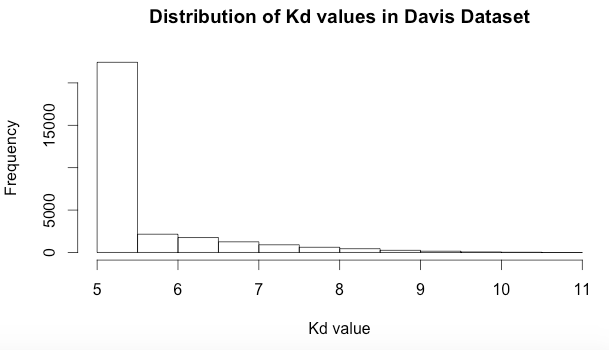
\includegraphics[scale=0.6]{davis_dist.png}
\end{center}
\caption{Distribution of $K_d$ values given in the Davis dataset.}
\label{fig:numStructure}
\end{figure}

\subsection{The Metz Dataset}

Just as the \textit{Davis} dataset, the continuous dataset \textit{Metz} was used for the evaluation of the drug-target interaction prediction model presented in \cite{pahikkala2014toward}. The dataset was published in the study \cite{metz2011navigating}. The \textit{Metz} dataset consists of 1421 drugs and 156 targets. The binding affinity is given as log transformed $K_i$ values for 42$\%$ of the drug-target pairs. As drug-drug and target-target similarities for this dataset the matrices were used that can be downloaded from the website of the author of \cite{pahikkala2014toward}.
\begin{figure}
\begin{center}
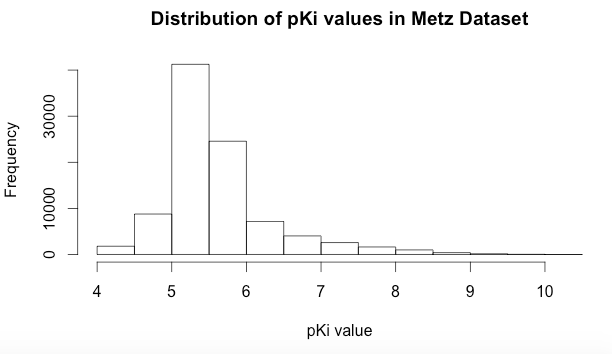
\includegraphics[scale=0.6]{metz_dist.png}
\end{center}
\caption{Distribution of $K_i$ values given in the Metz dataset.}
\label{fig:numStructure}
\end{figure}

\subsection{The KIBA Dataset}

The \textit{Davis} and \textit{Metz} datasets are suitable for the evaluation of predictive models for drug target interaction because data heterogeneity is not an issue. We can assume that the experimental settings for the measured drug target pairs in each dataset were the same and the binding affinities are comparable. When working with experimental results that come from multiple sources the data might be heterogeneous: In one case the binding affinity might be measured by $K_i$, in another case by $K_d$ and in a third case by $IC_{50}$ value. Another source of data heterogeneity are different experimental settings. An approach to integrate the observations from different sources, named \textit{KIBA} and a corresponding dataset is presented in \cite{tang2014making}. With their method, the authors of \cite{tang2014making} integrated the experimental results from multiple databases into a bioactivity matrix of 52498 compounds and 467 targets, including 246088 observations. The binding affinities in this matrix are given as \textit{KIBA}-scores. This dataset was used to obtain a third evaluation dataset, which is called the \textit{KIBA} dataset, by removing all drugs and targets with less than 10 observations from the original dataset that was downloaded from the supplementary material of \cite{tang2014making}, resulting in a dataset of 2116 drugs and 229 targets with a density of $~24\%$. For this dataset the drug-drug similarity matrix was computed through the PubChem structure clustering tool (https://pubchem.ncbi.nlm.nih.gov/assay/assay.cgi?p=clustering). The target target similarity matrix was computed by computing the normalized Smith Waterman Score \cite{yamanishi2010drug} for each pair of targets.

\begin{figure}
\begin{center}
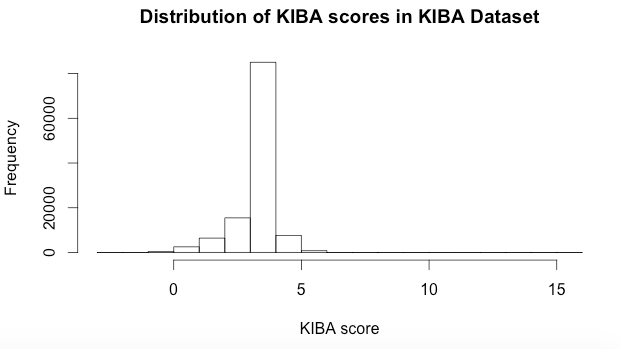
\includegraphics[scale=0.6]{kiba_dist.png}
\end{center}
\caption{Distribution of KIBA scores given in the KIBA dataset.}
\label{fig:numStructure}
\end{figure}


\section{Experimental Settings}

\subsection{Binary vs. Continuous Prediction}
\label{bincont}
For the evaluation of the model, a performance evaluation for the classification of drug-target pairs into binding or non-binding was also included, using the metrics \textit{AUC} and \textit{AUPR}. Therefore, the datasets where binarized by applying thresholds as it was done in \cite{pahikkala2014toward}. The $MF+CCRF$ model can only predict continuous values, therefore the threshold was applied on the true values after the prediction step, in order to compute $AUC$ and $AUPR$. In the \textit{Davis} and \textit{Metz} datasets, the higher the $pK_d$ or $pK_i$ value, the higher the binding affinity between a drug and a target. For the \textit{Metz} dataset, the same threshold of $pK_i\geq7.6$ was used as suggested in \cite{pahikkala2014toward} to assign a label of $1$ meaning binding and $0$ meaning non-binding. For the \textit{Davis} dataset, a threshold of $pK_d\geq7.0$ which is a bit less stringent than the threshold that is suggested in \cite{pahikkala2014toward} is used. In the original \textit{KIBA} dataset, the lower the \textit{KIBA}-score, the higher the binding affinity and \cite{tang2014making} suggests a threshold of \textit{KIBA}-score$\leq3$ to binarize the dataset. In an additional preprocessing step, the \textit{KIBA}-scores were transformed by taking the negative of each value and adding the minimum to all values in order to obtain a threshold where all values \textit{above} the threshold are classified as binding. The \textit{KIBA} threshold of $3$ in the un-transformed dataset then becomes $12.1$ in the transformed \textit{KIBA} dataset. 

It is noteworthy, that when the classification metrics $AUC$ and $AUPR$ are applied, $KronRLS$ learns and predicts binary labels, meaning that the datasets are binarized according to the cutoff thresholds before the training step. The $MF+CCRF$ method in contrast, only predicts continuous values and the cutoff threshold is applied after the prediction step to calculate the $AUC$ and $AUPR$. One can argue, that given two models $A$ and $B$, where $A$ learns to predict continuous values and model $B$ learns to predict binary values, and the performance of model $A$ in terms of $AUC$ and $AUPR$ is as good as the performance of model $B$, then model $A$ is advantageous because it does not need to be retrained (as model $B$) when the cutoff threshold for the dataset is changed.

\subsection{Performance Evaluation}
The model is evaluated using 5 fold cross-validation. In this procedure, the given values in the datasets are randomly partitioned into 5 subsets of equal size. Each subset is in turn used as validation data to test the method that was trained on the remaining 4 subsets. Both, the \textit{MF+CCRF} model and the comparison model $KronRLS$ can use as input either only one of the similarity metrics or both (in addition to the training matrix with the observed binding affinities). When $KronRLS$ gets as input only one of the similarity matrices for example only the drug similarity, it automatically generates a similarity kernel for the targets, where each target is only similar to itself, meaning the identity matrix is imputed for the targets (and vice-versa, when only the target-similarity is given, the identity matrix is used for the drugs). For each dataset, for each performance metric and for each method ($KronRLS$ and \textit{MF+CCRF}), we get 3 evaluation scores that can be compared among the two methods as illustrated in. For the \textit{MF+CCRF} model a fourth evaluation score is listed in the results section, which is the performance of using no similarity information, resulting in the prediction of only $MF$. The used performance metrics are described in the following sections. Figure \ref{fig:evaluation_tables} explains how to read the tables, listing the performance scores

\begin{figure}
\begin{center}
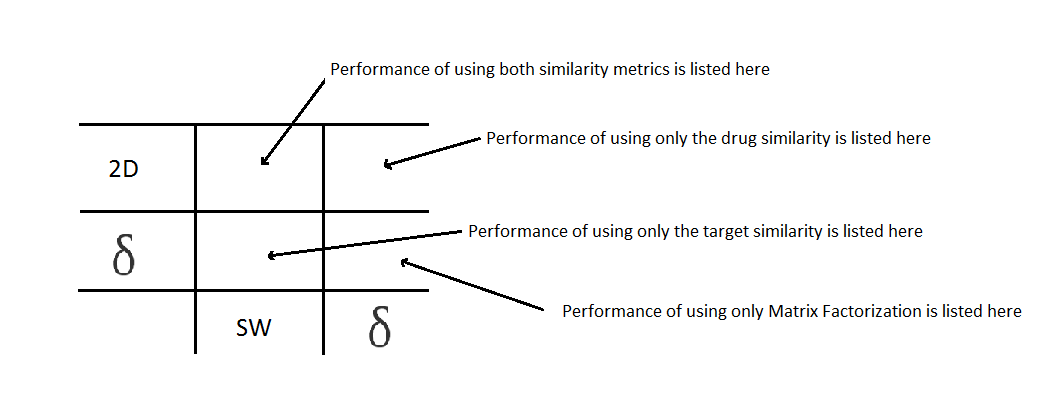
\includegraphics[scale=0.65]{evaluation_descr.png}
\end{center}
\caption[Description of evaluation tables]{\large{Description of the evaluation tables. 2D refers to the drug similarity (the drug similarity is based on the 2-dimensional structure of the compounds as described above). SW refers to the target similarity and stands for Smith-Waterman as described in the Dataset section. $\delta$ is used in the row/column where the drug/target similarity is not used.}}
\label{fig:evaluation_tables}
\end{figure}

\subsubsection{Evaluation Metrics}
As suggested in \cite{pahikkala2014toward}, the concordance index ($CI$) can be used as an evaluation metric for the prediction accuracy as it takes into account that the interaction affinities behind drug-target interactions are continuous values rather than binary ones. The intuition behind the $CI$ is as follows: the $CI$ over a set of paired data is the probability that the predictions for two randomly drawn drug-target pairs with different label values are in the correct order, meaning that the prediction $f_i$ for the larger affinity $y_i$ is larger than the prediction $f_j$ for the smaller affinity value $y_j$:

\begin{equation}
CI = \frac{1}{Z} \sum\limits_{y_i>y_j}h(f_i-f_j)
\end{equation}

where $Z$ is a normalization constant that equals the number of data pairs with different label values, and $h(u)$ is the step function returning $1.0$, $0.5$ and $0.0$ for $u>0$, $u=0$ and $u<0$ respectively. The $CI$ ranges between $0.5$ and $1.0$, where $0.5$ corresponds to a random predictor and $1.0$ corresponds to perfect prediction accuracy \cite{pahikkala2014toward}. 

As mentioned above, the datasets were also binarized according to cut-off thresholds to evalute the performance on the classification task. In case of binary interaction labels, the $CI$ becomes equal to the commonly used Area Under the Receiver Operating Characteristic Curve (AUC) metric \cite{pahikkala2014toward}:

\begin{equation}
AUC = \frac{1}{m_+m_-}\sum\limits_{y_i=1,y_j=-1}h(f_i-f_j)
\end{equation}

where $m_+$ and $m_-$ are the numbers of drug-target pairs belonging to the positive and negative classes. For the binary classification task, the performance was also evaluated using the Area Under the Precision-Recall curve (AUPR), which has been used in most of the previous studies on drug-target interaction prediction.




\chapter{Results}

List all results here


%   BACK MATTER  %%%%%%%%%%%%%%%%%%%%%%%%%%%%%%%%%%%%%%%%%%%%%%%%%%%%%%%%%%%%%%
%
%   References and appendices. Appendices come after the bibliography and
%   should be in the order that they are referred to in the text.
%
%   If you include figures, etc. in an appendix, be sure to use
%
%       \caption[]{...}
%
%   to make sure they are not listed in the List of Figures.
%

\backmatter%
	\addtoToC{Bibliography}
	\bibliographystyle{plain}
	\bibliography{references}

\end{document}
